% Chapter 4

\chapter{DATA PREPROCESSING} % Write in your own chapter title

For experimentation, the collection of Python programs compiled by the
Dublin City University \cite{A} on student code solutions for Python
assignments over 3 years was selected. Their data collection technique
involved students submitting their solutions to an online grading
platform where an auto grader reports as correct (Class 1) or as
incorrect (Class 0), based on success and failure of test cases,
respectively. Although this information is invaluable to instructors,
we aim to improve the representation of programs and consequently
improve the necessary recommendation provided. Attributing to the vast
size of the dataset and basing our task to an educational context
where student assignments are constantly being updated, we considered
a subset of 4 different programming questions to provide constructive
feedback. The shortlisted programs and descriptions for each are
listed in Table 4.1. For each task, 120 different code solutions were
randomly selected.  Overall, for the 4 different questions, 480 code
solutions were compiled for experimentation.

\begin{table}[H]
\caption{Questions and Description}
\centering
\resizebox{\textwidth}{!}{%
\begin{tabular}{|c|l|}
\hline
\textbf{Questions}        & \multicolumn{1}{c|}{\textbf{Description}}    \\ \hline
Selection sort            & Returns a sorted list from an unordered list \\ \hline
First negative element in a list    & Returns the first negative element in a list        \\ \hline
Unique characters count in a string & Returns a histogram of character counts in a string \\ \hline
Largest element of a list & Returns the largest element in a list        \\ \hline
\end{tabular}%
}

\label{tab:ques}
\end{table}

\section{DATASET ANNOTATION}

To model the dataset for the task of regression, we need
continuous values for the target variable. Considering the
derived dataset has categorical values (0 \& 1) for the
target variable, we devised a grading rubric to assign
numeric scores to respective code records. The numeric scores
are values in the range from 0 to 10 and they represent the
goodness of the code solutions to the particular
problem. Accordingly, higher numeric score represents a
correct and better code solution to the problem and lower
numeric score represents an incorrect or non-optimal code
solution.  Figure~4.1 represents the flowchart architecture
for dataset annotation.

\begin{figure}[h]
\centering
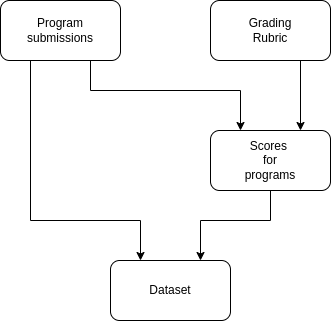
\includegraphics{./figures/data.png}
\caption{Data Annotation Flow}
\label{fig1}
\end{figure}

The score component for a value of 10 points was divided into
two parts namely \textbf{Design} (5 points) and
\textbf{Functionality} (5 points). The subsequent pattern
managed to cover the entirety of a code solution to provide a
value balancing the code's design and functionality.


For design, considering each problem has its own set of
parameters to satisfy, the grading rubric is adjusted based
on this requirement. The parameters used for evaluating
design is mentioned in Table~4.2. Tables~4.3 to 4.6 details
the appropriate score to respective problems based on their
necessary individual criteria for each different task.
        
        
\begin{table}[H]
\centering
\caption{Grading Parameters}
\begin{tabular}{|c|}
\hline
\emph{Parameters} \\ \hline
Use of Variables \\ \hline
Modularity \\ \hline
Logic Application \\ \hline
Efficiency \\ \hline
\end{tabular}

\label{tab:params}
\end{table}


\begin{itemize}
\item \textbf{Selection Sort}
  \begin{table}[h]
    \centering
    \caption{Grading Rubric (Design) for Selection Sort}
    \begin{tabular}{|l|c|}
      \hline
      \emph{Parameter}                                                          & \multicolumn{1}{l|}{\textbf{Weightage}} \\ \hline
      \begin{tabular}[c]{@{}l@{}}Code \\ modularity\\ \end{tabular}                  & 1                                       \\ \hline
      \begin{tabular}[c]{@{}l@{}}Use of \\ variables\\ \end{tabular}              & 1                                       \\ \hline
      \begin{tabular}[c]{@{}l@{}}The logic \\ applied\\ \end{tabular}             & 1                                       \\ \hline
      \begin{tabular}[c]{@{}l@{}}Efficient use \\ of functions\\ \end{tabular} & 2                                       \\ \hline
    \end{tabular}

    \label{ss_rub_design}
  \end{table}

  For ``Selection Sort'' task, three functions had to be
  defined: one for swapping, another to find the smallest
  element of the list from a given index, and yet another
  function for sorting which will use the other two
  functions. Hence, the definition of functions and use of
  function calls becomes the important parameter for design
  consideration.

\item \textbf{First Negative Element in List}

  \begin{table}[h!]
    \centering
    \caption{Grading Rubric (Design) for First Negative
      Element in List}
    \begin{tabular}{|l|c|}
      \hline
      \textbf{Parameter}                                                 & \multicolumn{1}{l|}{\textbf{Weightage}} \\ \hline
      \begin{tabular}[c]{@{}l@{}}Use of \\ variables\end{tabular}     & 1                                       \\ \hline
      \begin{tabular}[c]{@{}l@{}}The logic \\ applied\end{tabular}    & 2                                       \\ \hline
      \begin{tabular}[c]{@{}l@{}}Efficiency\\ of solution\end{tabular} & 2                                       \\ \hline
    \end{tabular}

    \label{fn_rub_design}
  \end{table}

  For ``First Negative Element in List'' task, there was no
  need of functions as it only requires a simple looping
  statement and a conditional statement to find the first
  negative element in the list. The important design
  parameter now was the logic applied to find the first
  negative element and the efficiency of the solution (for
  instance, the use of break statement after finding the
  first negative element).

\item \textbf{Largest Element in the List}

  \begin{table}[h!]
    \centering
    \caption{Grading Rubric (Design) for Largest Element in
      List task}
    \begin{tabular}{|l|c|}
      \hline
      \textbf{Parameter}                                                 & \multicolumn{1}{l|}{\textbf{Weightage}} \\ \hline
      \begin{tabular}[c]{@{}l@{}}Use of \\ variables\end{tabular}     & 2                                       \\ \hline
      \begin{tabular}[c]{@{}l@{}}The logic \\ applied\end{tabular}    & 1                                       \\ \hline
      \begin{tabular}[c]{@{}l@{}}Efficiency\\ of solution\end{tabular} & 2                                       \\ \hline
    \end{tabular}

    \label{la_rub_design}
  \end{table}

  For ``Largest Element in the List'' task, there was no need
  of functions again as it only requires a simple looping
  statement and a conditional statement to find and print the
  index of the largest element in the list. Here, the
  definition and use of variables was the important parameter
  along with the efficiency.

\item \textbf{Unique Character Count in String}

  \begin{table}[h!]
    \centering
    \caption{Grading Rubric (Design) for Unique Character
      Count in string}
    \begin{tabular}{|l|c|}
      \hline
      \textbf{Parameter}                                                 & \multicolumn{1}{l|}{\textbf{Weightage}} \\ \hline
      \begin{tabular}[c]{@{}l@{}}Use of \\ variables\end{tabular}     & 1                                       \\ \hline
      \begin{tabular}[c]{@{}l@{}}The logic \\ applied\end{tabular}    & 1                                       \\ \hline
      \begin{tabular}[c]{@{}l@{}}Code\\ Modularity\end{tabular}          & 1                                       \\ \hline
      \begin{tabular}[c]{@{}l@{}}Efficiency\\ of solution\end{tabular} & 2                                       \\ \hline
    \end{tabular}

    \label{uc_rub_design}
  \end{table}

  For ``Unique Character Count in String'' task, functions
  can be defined to check and ignore special characters, a
  function could be defined to count the unique tokens,
  etc. Thus, the code could be made modular.  Since this
  particular task could be solved in a variety of ways, the
  efficiency of the solution matters more.
\end{itemize}

% \begin{table}
% \centering
% \caption{Grading Rubric}
% \label{tab:rubric}
% \resizebox{\textwidth}{!}{%
% \begin{tabular}{|l|c|c|c|c|} 
% \cline{2-5}
% \multicolumn{1}{l|}{}                  & \multicolumn{4}{c|}{\begin{tabular}[c]{@{}c@{}}\textbf{}\\\textbf{Parameters}\\\textbf{}\end{tabular}}                                                                                                                                          \\ 
% \hline
% \multicolumn{1}{|c|}{\textbf{Program}} & \textit{\textbf{~ ~Use of Variables~~}} & \textit{\textbf{~ ~ Modularity~ ~~}} & \textit{\textbf{~ ~Logic application~~}} & \begin{tabular}[c]{@{}c@{}}\textit{\textbf{}}\\\textit{\textbf{~ ~Efficiency~ ~}}\\\textit{\textbf{}}\end{tabular}  \\ 
% \hline
% First Negative Element in List~ ~ ~ ~~ & 1                                       & -                                    & 2                                        & \begin{tabular}[c]{@{}c@{}}\\2\\\end{tabular}                                                                       \\ 
% \hline
% Selection Sort                         & 1                                       & 1                                    & 1                                        & \begin{tabular}[c]{@{}c@{}}\\2\\\end{tabular}                                                                       \\ 
% \hline
% Largest Element in List                & 1                                       & -                                    & 2                                        & \begin{tabular}[c]{@{}c@{}}\\2\\\end{tabular}                                                                       \\ 
% \hline
% Unique Count of Characters             & 1                                       & 1                                    & 1                                        & \begin{tabular}[c]{@{}c@{}}\\2\\\end{tabular}                                                                       \\
% \hline
% \end{tabular}%
% }
% \end{table}



% \begin{table}[h]
% \centering
% \label{tab:rubric}
% \resizebox{\textwidth}{!}{%
% \begin{tabular}{l|cccc|}
% \cline{2-5}
%  & \multicolumn{4}{c|}{\textbf{Parameters}} \\ \hline
% \multicolumn{1}{|c|}{\textbf{Program}} & \multicolumn{1}{l|}{\textit{\textbf{Use of Variables}}} & \multicolumn{1}{l|}{\textit{\textbf{Modularity}}} & \multicolumn{1}{l|}{\textit{\textbf{Logic application}}} & \multicolumn{1}{l|}{\textit{\textbf{Efficiency}}} \\ \hline
% \multicolumn{1}{|l|}{First Negative Element in List} & \multicolumn{1}{c|}{1} & \multicolumn{1}{c|}{-} & \multicolumn{1}{c|}{2} & 2 \\ \hline
% \multicolumn{1}{|l|}{Bank Account} & \multicolumn{1}{c|}{2} & \multicolumn{1}{c|}{1} & \multicolumn{1}{c|}{1} & 1 \\ \hline
% \multicolumn{1}{|l|}{Selection Sort} & \multicolumn{1}{c|}{1} & \multicolumn{1}{c|}{1} & \multicolumn{1}{c|}{1} & 2 \\ \hline
% \multicolumn{1}{|l|}{Largest Element in List} & \multicolumn{1}{c|}{1} & \multicolumn{1}{c|}{-} & \multicolumn{1}{c|}{2} & 2 \\ \hline
% \multicolumn{1}{|l|}{Unique Count of Characters} & \multicolumn{1}{c|}{1} & \multicolumn{1}{c|}{1} & \multicolumn{1}{c|}{1} & 2 \\ \hline
% \end{tabular}%
% }
% \caption{Grading Rubric}
% \end{table}

\newpage

For \textbf{functionality}, the following rubric mentioned in
Table~4.7 was followed to give a score in a scale of 5. The
correctness and completeness of the code was considered to
grade the code submissions.

\begin{table}[H]
\centering
\caption{Grading Rubric (Functionality)}
\begin{tabular}{|l|c|}
\hline
\textbf{\begin{tabular}[c]{@{}l@{}}Code's correctness\\ and \\ completeness\end{tabular}} & \multicolumn{1}{l|}{\textbf{Score}} \\ \hline
\begin{tabular}[c]{@{}l@{}}Perfectly correct\\ and complete\end{tabular}                     & 5                                   \\ \hline
\begin{tabular}[c]{@{}l@{}}Correct and complete\\ but can be improved\end{tabular}           & 4                                   \\ \hline
\begin{tabular}[c]{@{}l@{}}Complete but \\ partially incorrect\end{tabular}                  & 3                                   \\ \hline
\begin{tabular}[c]{@{}l@{}}Incomplete and\\ partially correct\end{tabular}                   & 2                                   \\ \hline
\begin{tabular}[c]{@{}l@{}}Incomplete and\\ totally incorrect\end{tabular}                   & 1                                   \\ \hline
\end{tabular}

\label{grading_rub}
\end{table}

Finally, a dataset compiled of code solutions and appropriate
numeric score values (in the range from 0 to 10) was
generated to be used for the subsequent experimentation.

\newpage

\subsection{Example Code Submissions}

Figures~4.2 to 4.9 document the examples of best and worst
programs for each problem with scores assigned using the
developed grading rubric.

\subsubsection{Selection Sort}

\begin{figure}[h]
\centering
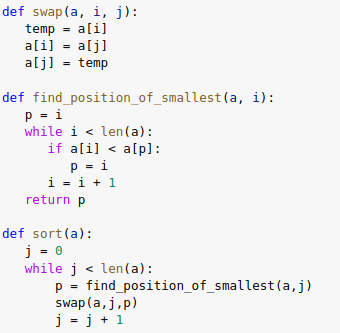
\includegraphics[]{./figures/best_ss.png}
\caption{Best Program - Selection Sort}
\label{fig1}
\end{figure}

\begin{figure}[H]
\centering
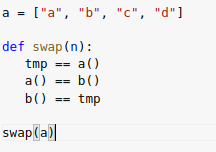
\includegraphics[scale=1.2]{./figures/ss_worst.png}
\caption{Worst Program - Selection Sort}
\label{fig1}
\end{figure}


Figures 4.2 is one of the best program submissions for the
selection sort task. The program was properly structured with
three functions, one to do swapping, one to find smallest
element's position from a given index from the list, and
finally the sort function which will utilise the first two
functions inside a loop to sort the list. Hence, it was
awarded a perfect 10/10.

Figure 4.3 is one of the worst program submissions. This code
solution has a swap function defined but with wrong logic. A
unnecessary global variable 'a' was declared. The logic of
the swap function was not right. Hence this solution was
graded 1/10.

\newpage
\subsubsection{First negative element in a list}

\begin{figure}[h]
\centering
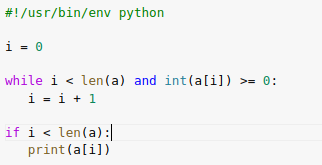
\includegraphics{./figures/best_fn.png}
\caption{Best Program - First negative element in a list}
\label{fig1}
\end{figure}

\begin{figure}[h]
\centering
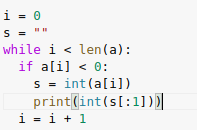
\includegraphics{./figures/worst_fn.png}
\caption{Worst Program - First negative element in a list}
\label{fig1}
\end{figure}

Figure~4.4 shows a good solution for finding the first
negative element in the list. The loop traverses the list
until it finds the first negative element. When that index
belongs to the list, the program prints the first negative
element. The program is graded a perfect 10/10.

Figure~4.5 shows one of the bad code solutions submitted. The
program is graded only 3/10 for using wrong logic and also
for improper declaration and use of variables.

\newpage

\subsubsection{Unique characters count in a string}

\begin{figure}[h]
\centering
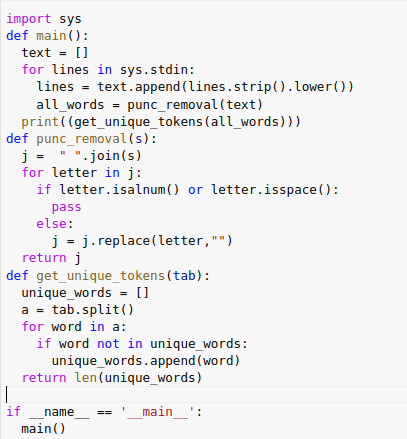
\includegraphics{./figures/best_uc.png}
\caption{Best Program - Unique characters count in a string}
\label{fig1}
\end{figure}

\newpage

\begin{figure}[H]
\centering
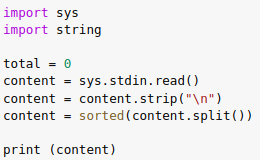
\includegraphics{./figures/worst_uc.png}
\caption{Worst Program - Unique characters count in a string}
\label{fig1}
\end{figure}

Figure 4.6 is one of the best program submissions for the
unique character count task. The code is properly organised,
modular with three functions and the code has perfect
logic. No unnecessary global variable is defined. Thus, this
particular submission was awarded with the perfect score of
10.

Figure 4.7 on the other hand shows one of the worst
submissions for this particular task. No functions have been
defined. An unnecessary global variable was declared. The
code would not yield the expected result. Thus, this code was
only given a score of 1.

\newpage

\subsubsection{Largest element of a list}

\begin{figure}[h]
\centering
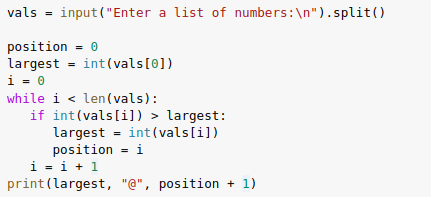
\includegraphics{./figures/best_la.png}
\caption{Best Program - Largest element of a list}
\label{fig1}
\end{figure}

\begin{figure}[h]
\centering
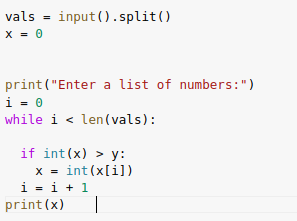
\includegraphics{./figures/worst_la.png}
\caption{Worst Program - Largest element of a list}
\label{fig1}
\end{figure}

\newpage

Figure 4.8 is one of the best student code submissions for
the largest element task. This particular solution has the
right logic.  Variables have been used properly. The program
prints the correct position of the largest element in the
list. Looping and conditional statements have been used
correctly. Thus, this solution was awarded as score of 10.

Figure 4.9 is one of the worst student submissions for this
task. Variables have not been properly used. The logic used
is also wrong. Hence, this code solution was only given a
score of 2.

\newpage

\section{FEATURE EXTRACTION}

Following the annotation of the dataset, feature extraction
and feature selection are performed for optimal
representation of code solutions as vectors for
regression. The following series of steps were performed for
extracting meaningful features from the dataset.

\begin{itemize}
\item \textbf{Py2 to Py3 conversion}: The code solutions in
  the dataset are documented in Python 2 version. To support
  extraction of features, Python 2 to Python 3 conversion was
  performed using the '2to3' module \cite{G}.
\item \textbf{Abstract Syntax Tree (AST) representation}:
  After converting every program to Python 3 format, the AST
  \cite{F} representation for each program was computed to
  derive appropriate features. The inbuilt Python `ast'
  module was used to get the ast representation of the
  student submissions. The `ast' module provides a `parse()'
  method which returns the AST representation of a program. A
  variety of features can be extracted from this ast
  representation with the help of `walk()' function provided
  by the `ast' module. The extracted features from the AST
  representation are documented in Table~4.9. Other features
  derived from code are represented in Table~4.8.
\end{itemize}

\begin{table}[H]
\centering
\caption{Features extracted from code}
\begin{tabular}{|l|l|} 
\hline
return       & Count of 'return' statements in the code      \\ 
\hline
break        & Count of 'break' statements in the code       \\ 
\hline
continue     & Count of 'continue' statements in the code    \\ 
\hline
pass         & Count of 'pass' statements in the code        \\ 
\hline
assign       & Count of assignment operators in the code     \\ 
\hline
arith        & Count of arithmetic operators in the code     \\ 
\hline
comp         & Count of comparison operators in the code     \\ 
\hline
log          & Count of logical operators in the code        \\ 
\hline
cond         & Count of conditional operators in the code    \\ 
\hline
loop         & Count of 'for' and 'while' loops in the code  \\ 
\hline
\#lines      & Count of lines in the code                    \\ 
\hline
\end{tabular}
\end{table}

\begin{table}[H]
\centering
\caption{Features extracted from AST} 
\begin{tabular}{|l|l|} 
\hline 
\#fun                 & Count of function definitions in the code                                                                                      \\ 
\hline
\#fcall               & Count of function calls in the code                                                                                            \\ 
\hline
globals               & Count of globals variables in the code                                                                                         \\ 
\hline
\#lst                 & Count of lists and tuples in the code                                                                                          \\ 
\hline
\#var                 & \begin{tabular}[c]{@{}l@{}}Count of the variables in the code\\(Count of variables defined)\end{tabular}                       \\ 
\hline
\#var\_uses           & \begin{tabular}[c]{@{}l@{}}Count of variable uses in the code\\(Count of variables used in different statements)\end{tabular}  \\ 
\hline
\end{tabular}
\end{table}


Ultimately a total of 17 features were extracted from the
code and the AST representation of the code.

\newpage
\section{FEATURE SELECTION}

After extracting meaningful features from both the code and
AST representation (Table~4.8, Table~4.9), feature
selection is performed for each problem considering feature
sets for each problem are independent of each other and are
problem dependent.

Firstly, the features that share the same value for all the
code solutions are identified and removed to avoid
redundancy. Once the redundant features are reduced, the
number of features eventually reduces from
\begin{itemize}
\item 17 to 14 for 'Selection sort'
\item 17 to 12 for 'The First negative element in the list'
\item 17 to 12 for 'The Largest Element in List'
\item 17 to 15 for 'The unique character count in a string
  task.'
\end{itemize}
Then, the best features are selected for each task according
to how well they are correlated with the target variable. The
\emph{f\_regression} method \cite{H} returns the degree of
correlation (F-statistic) between each feature and the
target.

The correlation F-statistic score of different features for
the tasks are listed as tables below. After the F-statistic
score is calculated, the features which have significant
influence on the target variable(score) are selected and the
regressor model for each task is trained with the selected
features.

\subsection{Implementation}

Tables~4.10 to 4.14 report the F-Statistic score of the
features set with their respective scores. The strike-through
text in features list of the tables represent the features
that are dropped due to their low $f{reg}$ score.

\begin{itemize}
\item \textbf{Selection Sort}
  \begin{table}[H]
    \centering
    \caption{F-statistic table : Selection Sort}
    \begin{tabular}{|l|l|}
      \hline
      \textbf{Feature} & \textbf{$f{reg}$ score} \\ \hline
      \#fun            & 387.16                \\ \hline
      loop             & 181.29                \\ \hline
      \#fcall          & 179.15                \\ \hline
      \#var\_uses      & 122.33                \\ \hline
      comp             & 104.35                \\ \hline
      \#lines          & 91.83                 \\ \hline
      return           & 91.55                 \\ \hline
      arith            & 68.54                 \\ \hline
      assign           & 65.93                 \\ \hline
      \#var            & 56.68                 \\ \hline
      cond             & 50.10                 \\ \hline
      \#lst            & 20.39                 \\ \hline
      globals          & 15.75                 \\ \hline
      \st{log}              & 1.81                  \\ \hline
    \end{tabular}
            
    \label{ss_f}
  \end{table}
            
  From Table 4.10, it can be observed that for 'Selection
  sort' task, the number of functions, loops, function calls,
  variable uses and comparison operators have a very strong
  correlation with the output score. The first 13 features
  have a considerably big influence on the target variable
  when compared to that of number of logical operators.
            
\item \textbf{First Negative Element in List}

  \begin{table}[H]
    \centering
    \caption{F-statistic table : First Negative Element in
      List}
    \begin{tabular}{|l|l|}
      \hline
      \textbf{Feature} & \textbf{$f{reg}$ score} \\ \hline
      comp             & 31.42                 \\ \hline
      \#var\_uses      & 6.33                  \\ \hline
      cond             & 6.02                  \\ \hline
      log              & 2.11                  \\ \hline
      assign           & 2.02                  \\ \hline
      loop             & 1.85                  \\ \hline
      break            & 1.49                  \\ \hline
      \#lines          & 1.47                  \\ \hline
      \#var            & 1.32                  \\ \hline
      \#lst            & 1.01                  \\ \hline
      \st{globals}          & 0.50                  \\ \hline
      \st{arith}            & 0.05                  \\ \hline

    \end{tabular}

    \label{fn_f}
  \end{table}

  From Table 4.11, it is observed that for the 'First
  negative element in the list' task, the number of
  comparison statements have a large correlation on the
  output variable. The number of variable uses and the number
  of conditional statements also have a good influence with
  the target variable. Here with a minimum cutoff of a F-reg
  score of 1, top 10 features become the selected features.

\newpage

\item \textbf{Largest Element in List}

\begin{table}[H]
\centering
\caption{F-statistic table : Largest Element in List}
\begin{tabular}{|l|l|}
\hline
\textbf{Feature} & \textbf{$f{reg}$ score} \\ \hline
assign           & 17.51                 \\ \hline
arith            & 15.91                 \\ \hline
\#var\_uses      & 12.47                 \\ \hline
globals          & 9.47                  \\ \hline
\#lst            & 3.82                  \\ \hline
comp             & 3.35                  \\ \hline
cond             & 3.35                  \\ \hline
\#var            & 2.49                  \\ \hline
\st{loop}             & 0.90                  \\ \hline
\st{break}            & 0.84                  \\ \hline
\st{\#lines}          & 0.73                  \\ \hline
\st{log}              & 0.02                  \\ \hline

\end{tabular}

\label{la_f}
\end{table}

From Table 4.12, it is observed for the 'Largest element in
the list' task, the number of assignment statements,
arithmetic operators and variable uses have a great influence
on the final target value. With a minimum cutoff of a F-reg
score 1.0 the top 8 features are selected.

\newpage

\item \textbf{Unique Character Count in List}

\begin{table}[H]
\centering
\caption{F-statistic table : Unique Character Count in List}
\begin{tabular}{ll}
\hline
\multicolumn{1}{|l|}{\textbf{Feature}} & \multicolumn{1}{l|}{\textbf{$f{reg}$ score}} \\ \hline
\multicolumn{1}{|l|}{log}              & \multicolumn{1}{l|}{15.76}                 \\ \hline
\multicolumn{1}{|l|}{\#fcall}          & \multicolumn{1}{l|}{4.94}                  \\ \hline
\multicolumn{1}{|l|}{\#var}            & \multicolumn{1}{l|}{3.58}                  \\ \hline
\multicolumn{1}{|l|}{cond}             & \multicolumn{1}{l|}{3.52}                  \\ \hline
\multicolumn{1}{|l|}{pass}             & \multicolumn{1}{l|}{3.42}                  \\ \hline
\multicolumn{1}{|l|}{\#var\_uses}      & \multicolumn{1}{l|}{3.22}                  \\ \hline
\multicolumn{1}{|l|}{\#lst}            & \multicolumn{1}{l|}{2.91}                  \\ \hline
\multicolumn{1}{|l|}{loop}             & \multicolumn{1}{l|}{1.91}                  \\ \hline
\multicolumn{1}{|l|}{\st{return}}           & \multicolumn{1}{l|}{0.95}                  \\ \hline
\multicolumn{1}{|l|}{\st{comp}}             & \multicolumn{1}{l|}{0.78}                  \\ \hline
\multicolumn{1}{|l|}{\st{\#fun}}            & \multicolumn{1}{l|}{0.46}                  \\ \hline
\multicolumn{1}{|l|}{\st{\#lines}}          & \multicolumn{1}{l|}{0.34}                  \\ \hline
\multicolumn{1}{|l|}{\st{globals}}         & \multicolumn{1}{l|}{0.20}                  \\ \hline
\multicolumn{1}{|l|}{\st{arith}}            & \multicolumn{1}{l|}{0.17}                  \\ \hline
\multicolumn{1}{|l|}{\st{assign}}           & \multicolumn{1}{l|}{0.05}      
\\ \hline
\end{tabular}

\label{uc_f}
\end{table}

From Table 4.13, it is observed for the unique character
count in a string, the number of logical operators has the
highest influence on the final target output. This is due to
the number of 'not' and 'not in' operators. With a minimum
cutoff set at a F-reg score of 1.0, only the first eight
features are selected.
\end{itemize}